\section{Динамик баннерийн CRUD форм}
\subsection{Өгөгдлийн сан руу баннерийн CRUD хийх custom hook}
Database-с баннерийн өгөгдлийг унших, өөрчлөх, устгах болон шинээр үүсгэхэд хялбарчлах үүднээс custom hook бичсэн. Custom hook-н нэр нь "use" гэж эхэлсэн дахин ашиглах боломжтой функц бөгөөд бусад react hook-үүдийг дуудаж ажиллуулах боломжтой байдаг.

\lstinputlisting[language=Javascript, basicstyle=\linespread{0.8}\ttfamily, caption={Баннерийн CRUD хийх custom hook},frame=single]{src/code/banner/useBanner.js}

\subsection{Баннерийн форм validation хийх}
Энэхүү системд Yup хэмээх форм validation хялбарчлах зорилготой нэмэлт package-г ашигладаг. Yup-ийн тусламжтайгаар та өөрийн өгөгдлийн схемийг тодорхойлж, дараа нь өгөгдөл тухайн схемд нийцэж байгаа эсэхийг шалгадаг.
Форм validation нь вэб хөгжүүлэлтийн чухал хэсэг бөгөөд хэд хэдэн чухал зорилготой:
\begin{itemize}
   \item Формоор илгээсэн өгөгдөл хүлээгдэж буй шалгуур, чанарын стандартад нийцэж байгаа эсэхийг баталгаажуулах. Энэ нь буруу эсвэл бүрэн бус өгөгдлийг өгөгдлийн санд хадгалах эсвэл сервер рүү илгээхээс урьдчилан сэргийлэхэд тусалдаг.

   \item Хэрэглэгчдэд формоо илгээхээсээ өмнө буруу оруулсан мэдээллээ засч залруулахад тусалдаг.

   \item Бталгаажуулалт нь таны програмыг SQL injection эсвэл сайт хоорондын скрипт (XSS) гэх мэт хортой халдлагаас хамгаалахад тусалдаг.

   \item Серверийн ачааллыг бууруулах, шаардлагагүй хүсэлтийг бууруулдаг.
\end{itemize}
\lstinputlisting[language=Javascript, basicstyle=\linespread{0.8}\ttfamily, caption={Баннерийн форм validation},frame=single]{src/code/banner/bannerSchema.js}

\subsection{Фронтэнд хөгжүүлэлт}
Орчин цагийн Фронтэнд хөгжүүлэлтэнд хамгийн түгээмэл ашиглагддаг филсофи бол бүрэлдэхүүн хэсгүүдийг аль болох олон жижиг хэсгүүдэд хувааж дараа нь тэдгээрийг ахин ашиглах явдал юм.

Хэрэглэгч үндсэн, нэмэлт, контент гэсэн 3 төрлийн баннер үүсгэх боломжтой ба үндсэн болон нэмэлт хэдэн ч баннер үүсгэх боломжтой, харин ганц л контент баннер үүсгэх боломжтой байна.

Хэрэглэгч үүсгэсэн байгаа баннеруудаа харах боломжтой байх үүднээс баннерийн жагсаалт компонентыг бичиж өгсөн. Мөн хэрэглэгч баннер шинээр үүсгэх эсвэл шинэчлэх үед баннерийн форм компонентийг дуудна. Баннерийн формийг дуудах үед URL-н параметрт id байвал тухайн id-тай баннер мэдээллийг авч формийн оролтуудад бичнэ. Үүний дараагаар хэрэглэгч өөрийн хүссэн мэдээллээ шинэчлэх боломжтой болно.
\subsubsection{Баннерийн форм компонент}
\lstinputlisting[language=Javascript, basicstyle=\linespread{0.8}\ttfamily, caption={Баннерийн форм компонент},frame=single]{src/code/banner/BannerForm.js}
\subsubsection{Баннерийн жагсаалт компонент}
\lstinputlisting[language=Javascript, basicstyle=\linespread{0.8}\ttfamily, caption={Баннерийн жагсаалт компонент},frame=single]{src/code/banner/BannerList.js}

\subsection{Үр дүн}
Хэрэгжүүлэлтийн үр дүн:
\begin{figure}
	\centering
	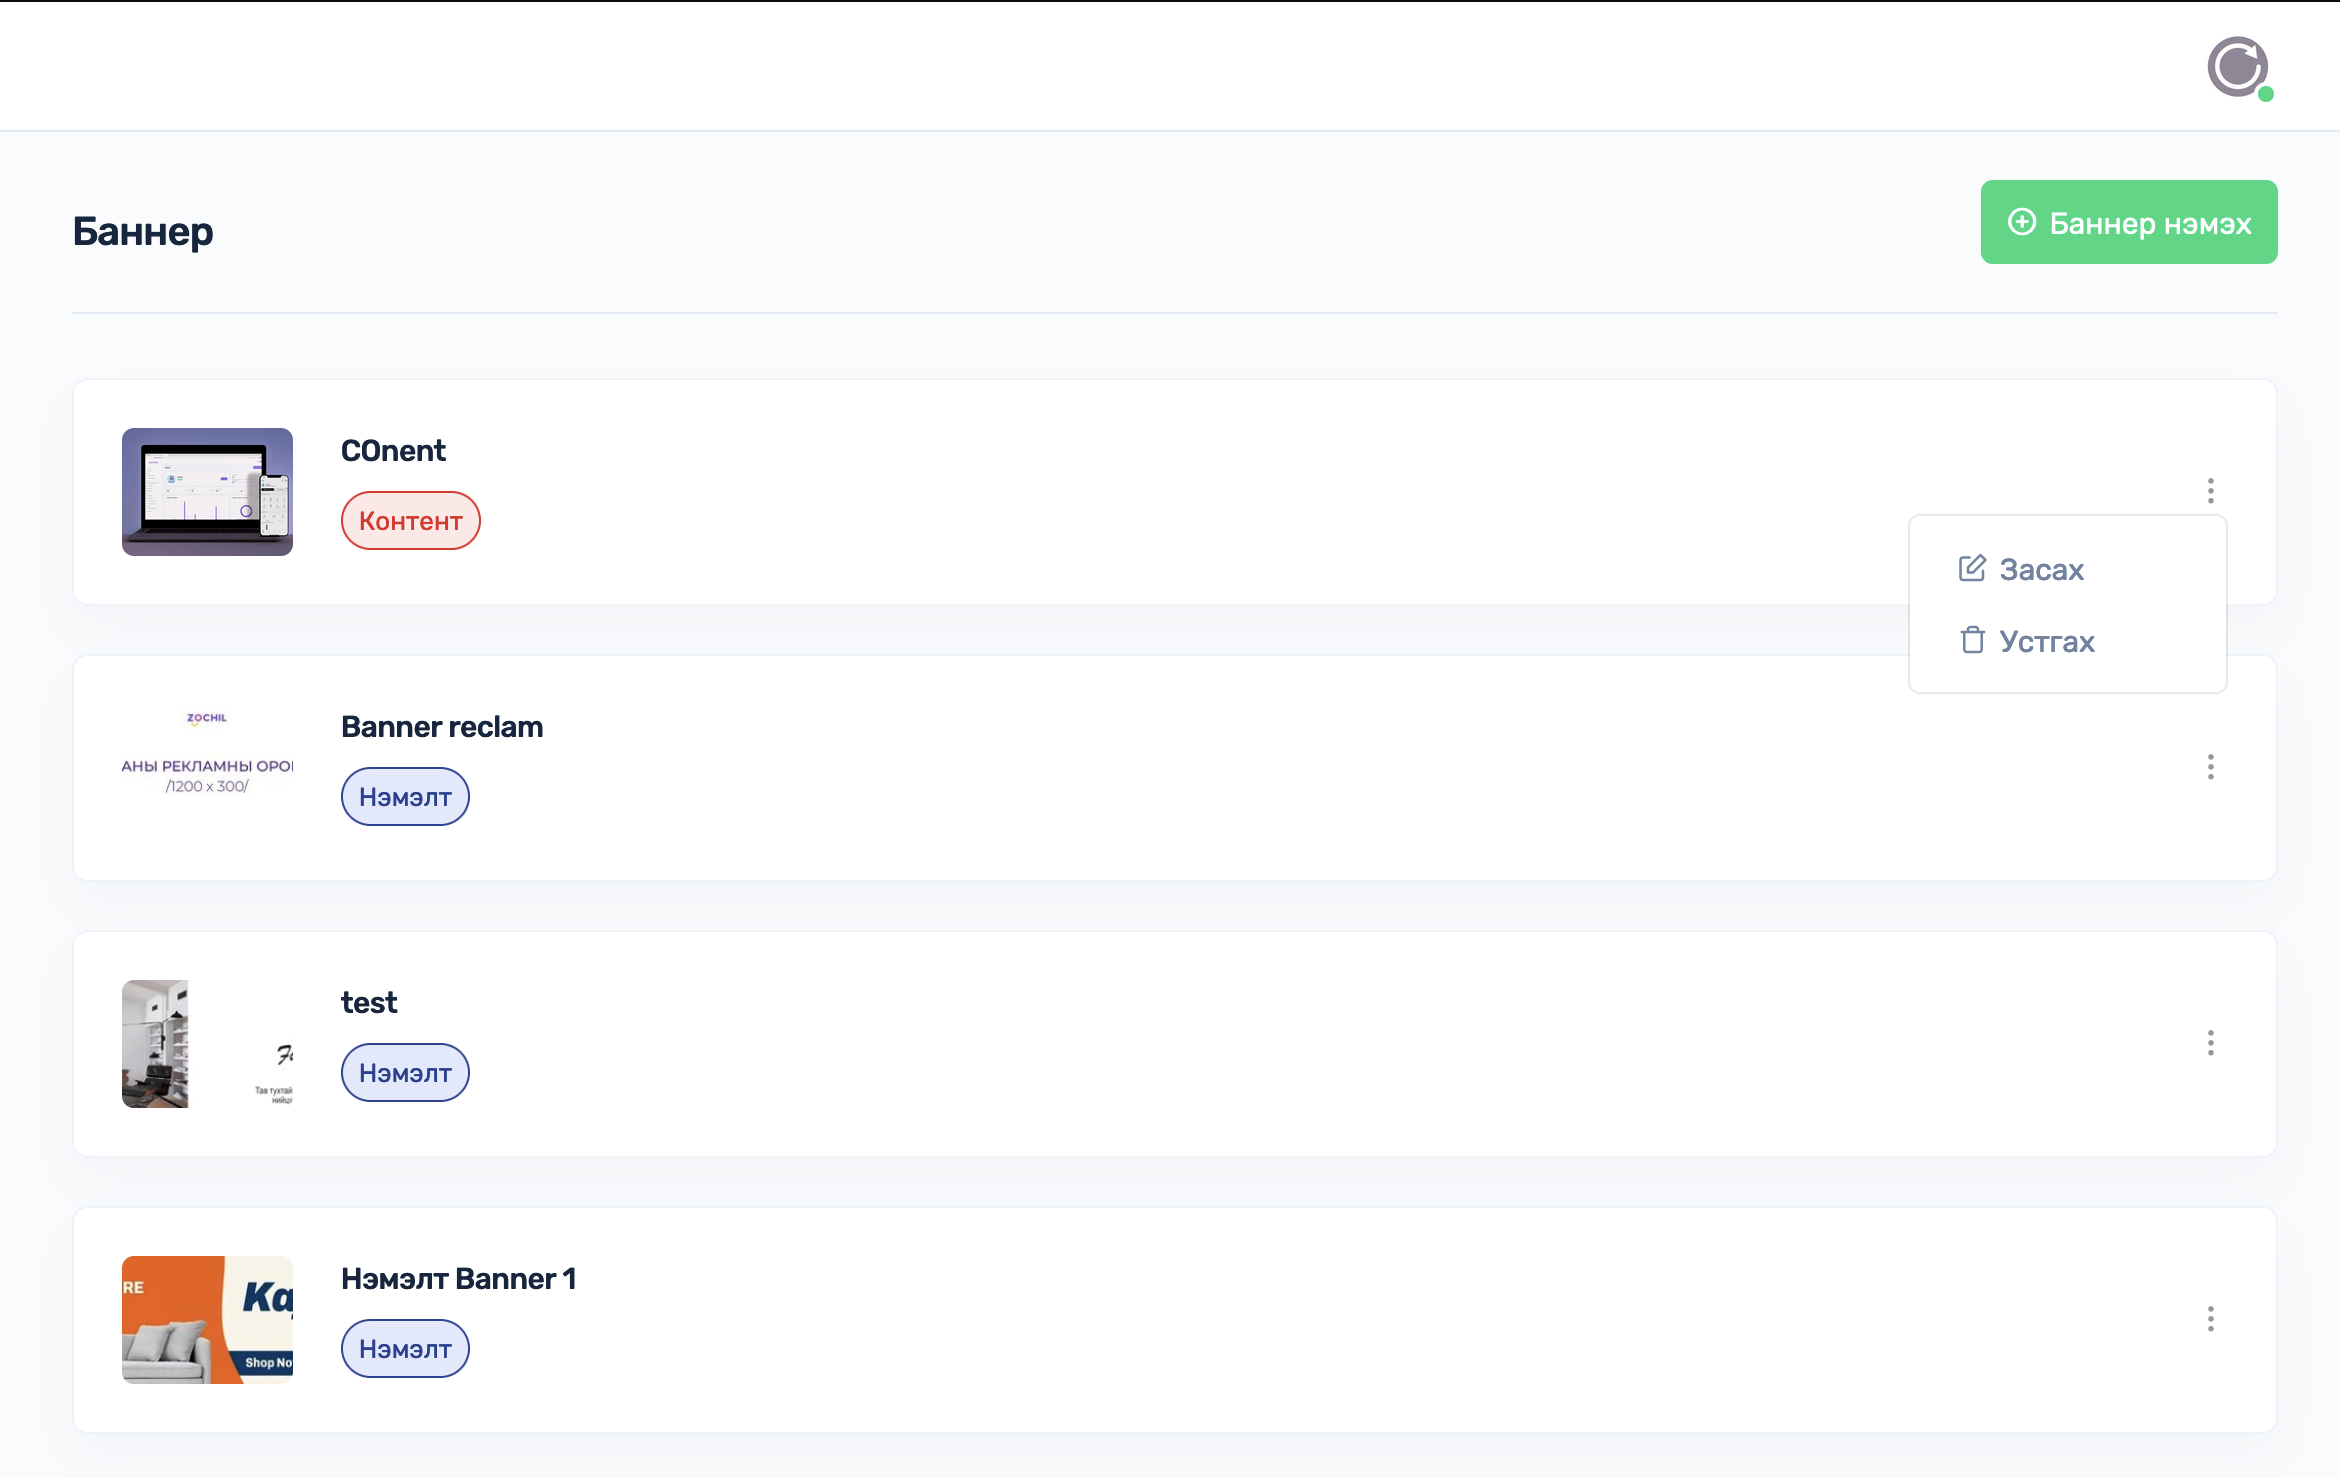
\includegraphics[scale=0.15]{src/images/banner-list.png}
	\caption{Баннерийн жагсаалт хэсэг}
\end{figure}
\begin{figure}
	\centering
	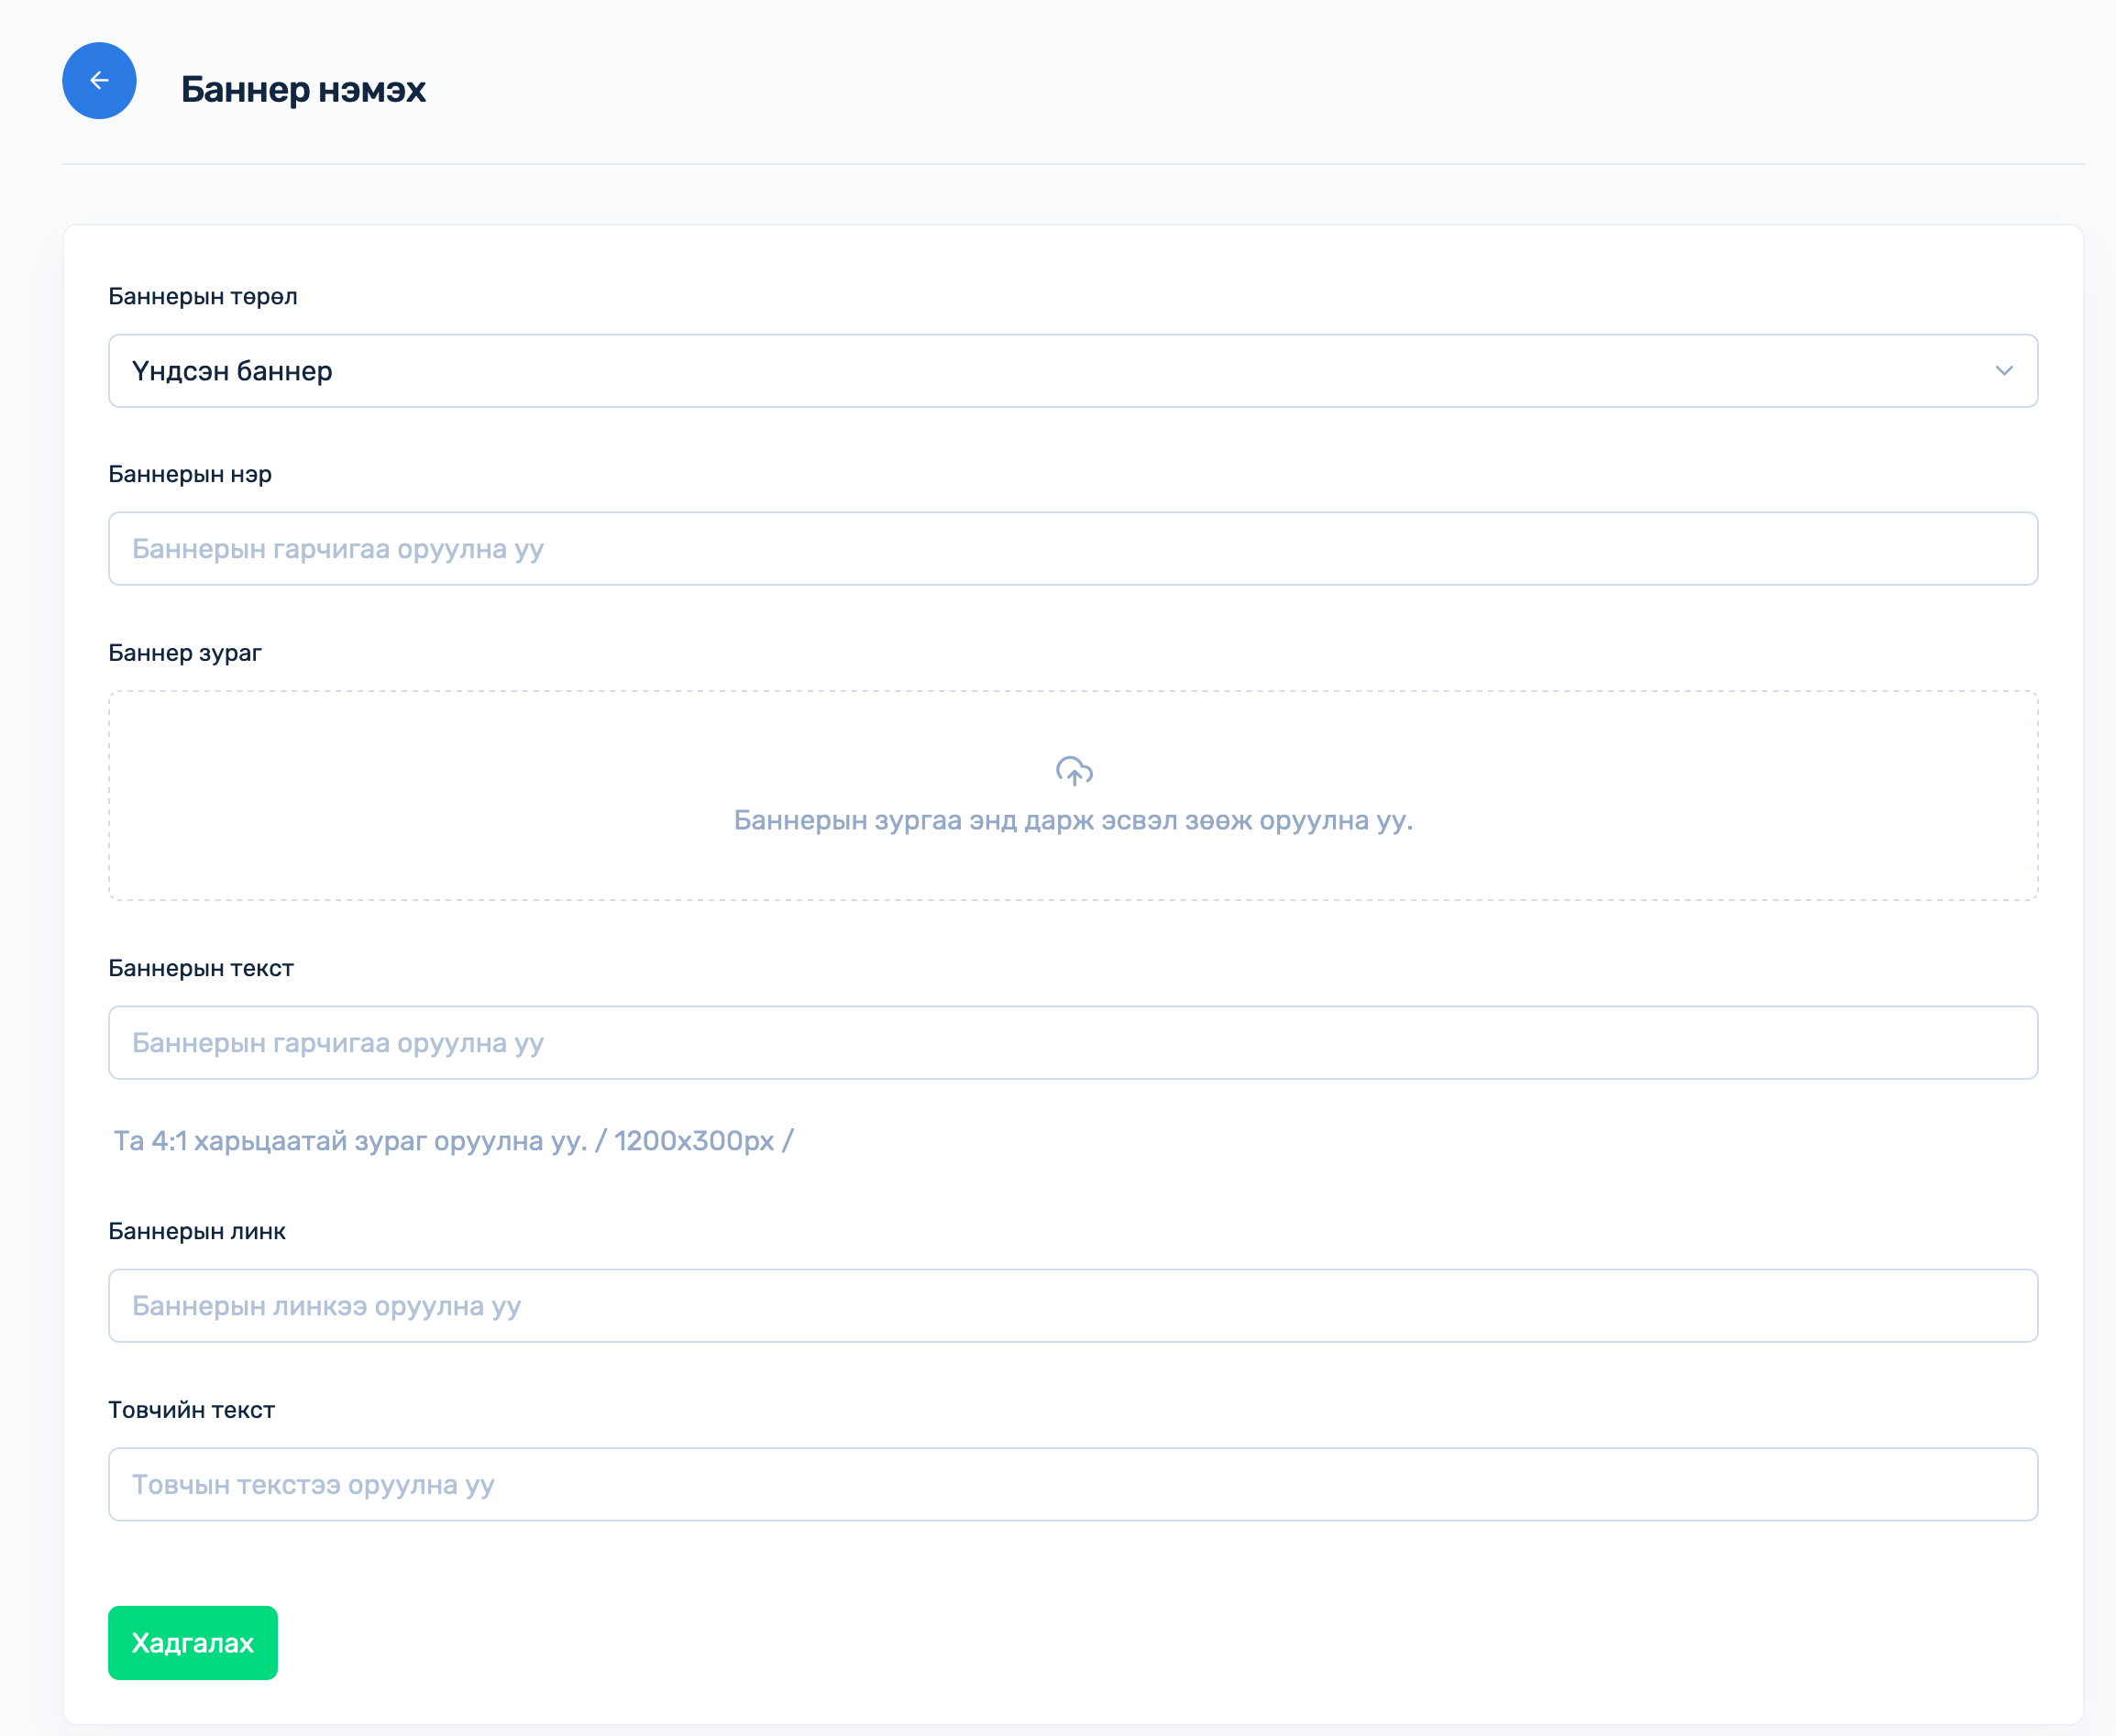
\includegraphics[scale=0.15]{src/images/banner-form.png}
	\caption{Баннерийн форм хэсэг}
\end{figure}


\section{Арга хэмжээ үүсгэх CRUD форм}
\subsection{Өгөгдлийн сан руу арга хэмжээг CRUD хийх custom hook}
\lstinputlisting[language=Javascript, basicstyle=\linespread{0.8}\ttfamily, caption={Арга хэмжээн CRUD хийх custom hook},frame=single]{src/code/event/useEvent.js}

\subsection{Арга хэмжээн форм validation хийх}
\lstinputlisting[language=Javascript, basicstyle=\linespread{0.8}\ttfamily, caption={Арга хэмжээн форм validation},frame=single]{src/code/event/eventSchema.js}

\subsection{Фронтэнд хөгжүүлэлт}
\subsubsection{Арга хэмжээн форм компонент}
\lstinputlisting[language=Javascript, basicstyle=\linespread{0.8}\ttfamily, caption={Арга хэмжээн форм компонент},frame=single]{src/code/event/EventForm.js}
\subsubsection{Арга хэмжээн жагсаалт компонент}
\lstinputlisting[language=Javascript, basicstyle=\linespread{0.8}\ttfamily, caption={Арга хэмжээн жагсаалт компонент},frame=single]{src/code/event/EventList.js}

\subsection{Үр дүн}
\begin{figure}[h]
	\centering
	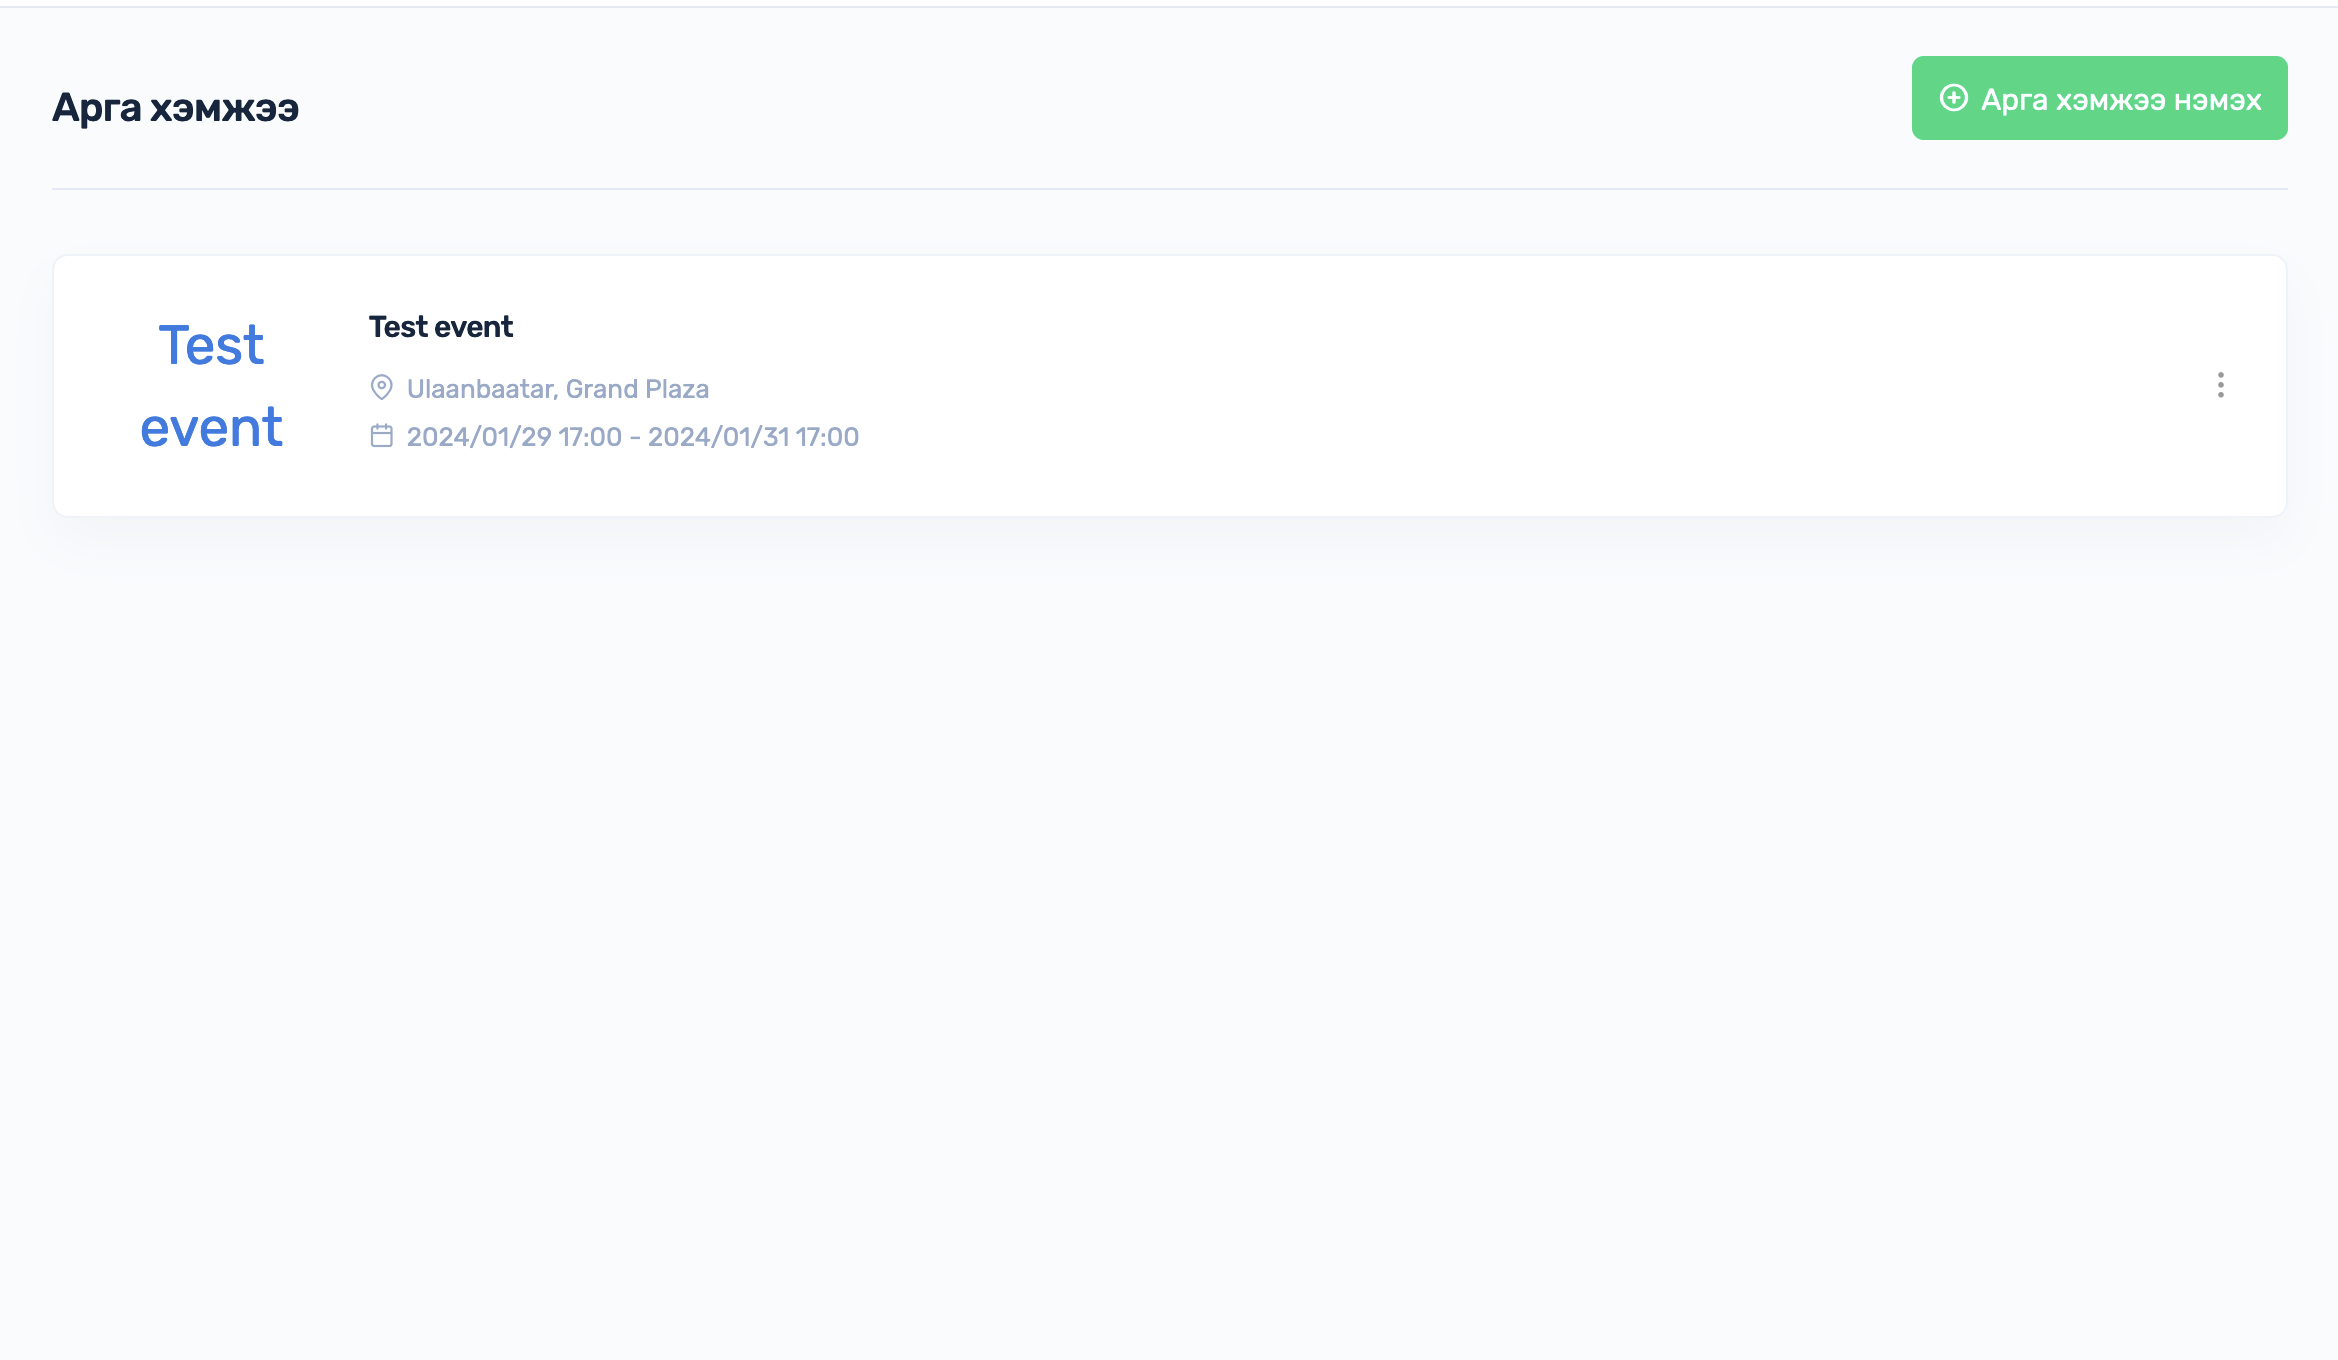
\includegraphics[scale=0.2]{src/images/event-list.png}
	\caption{Баннерийн жагсаалт хэсэг}
\end{figure}
\begin{figure}[h]
	\centering
	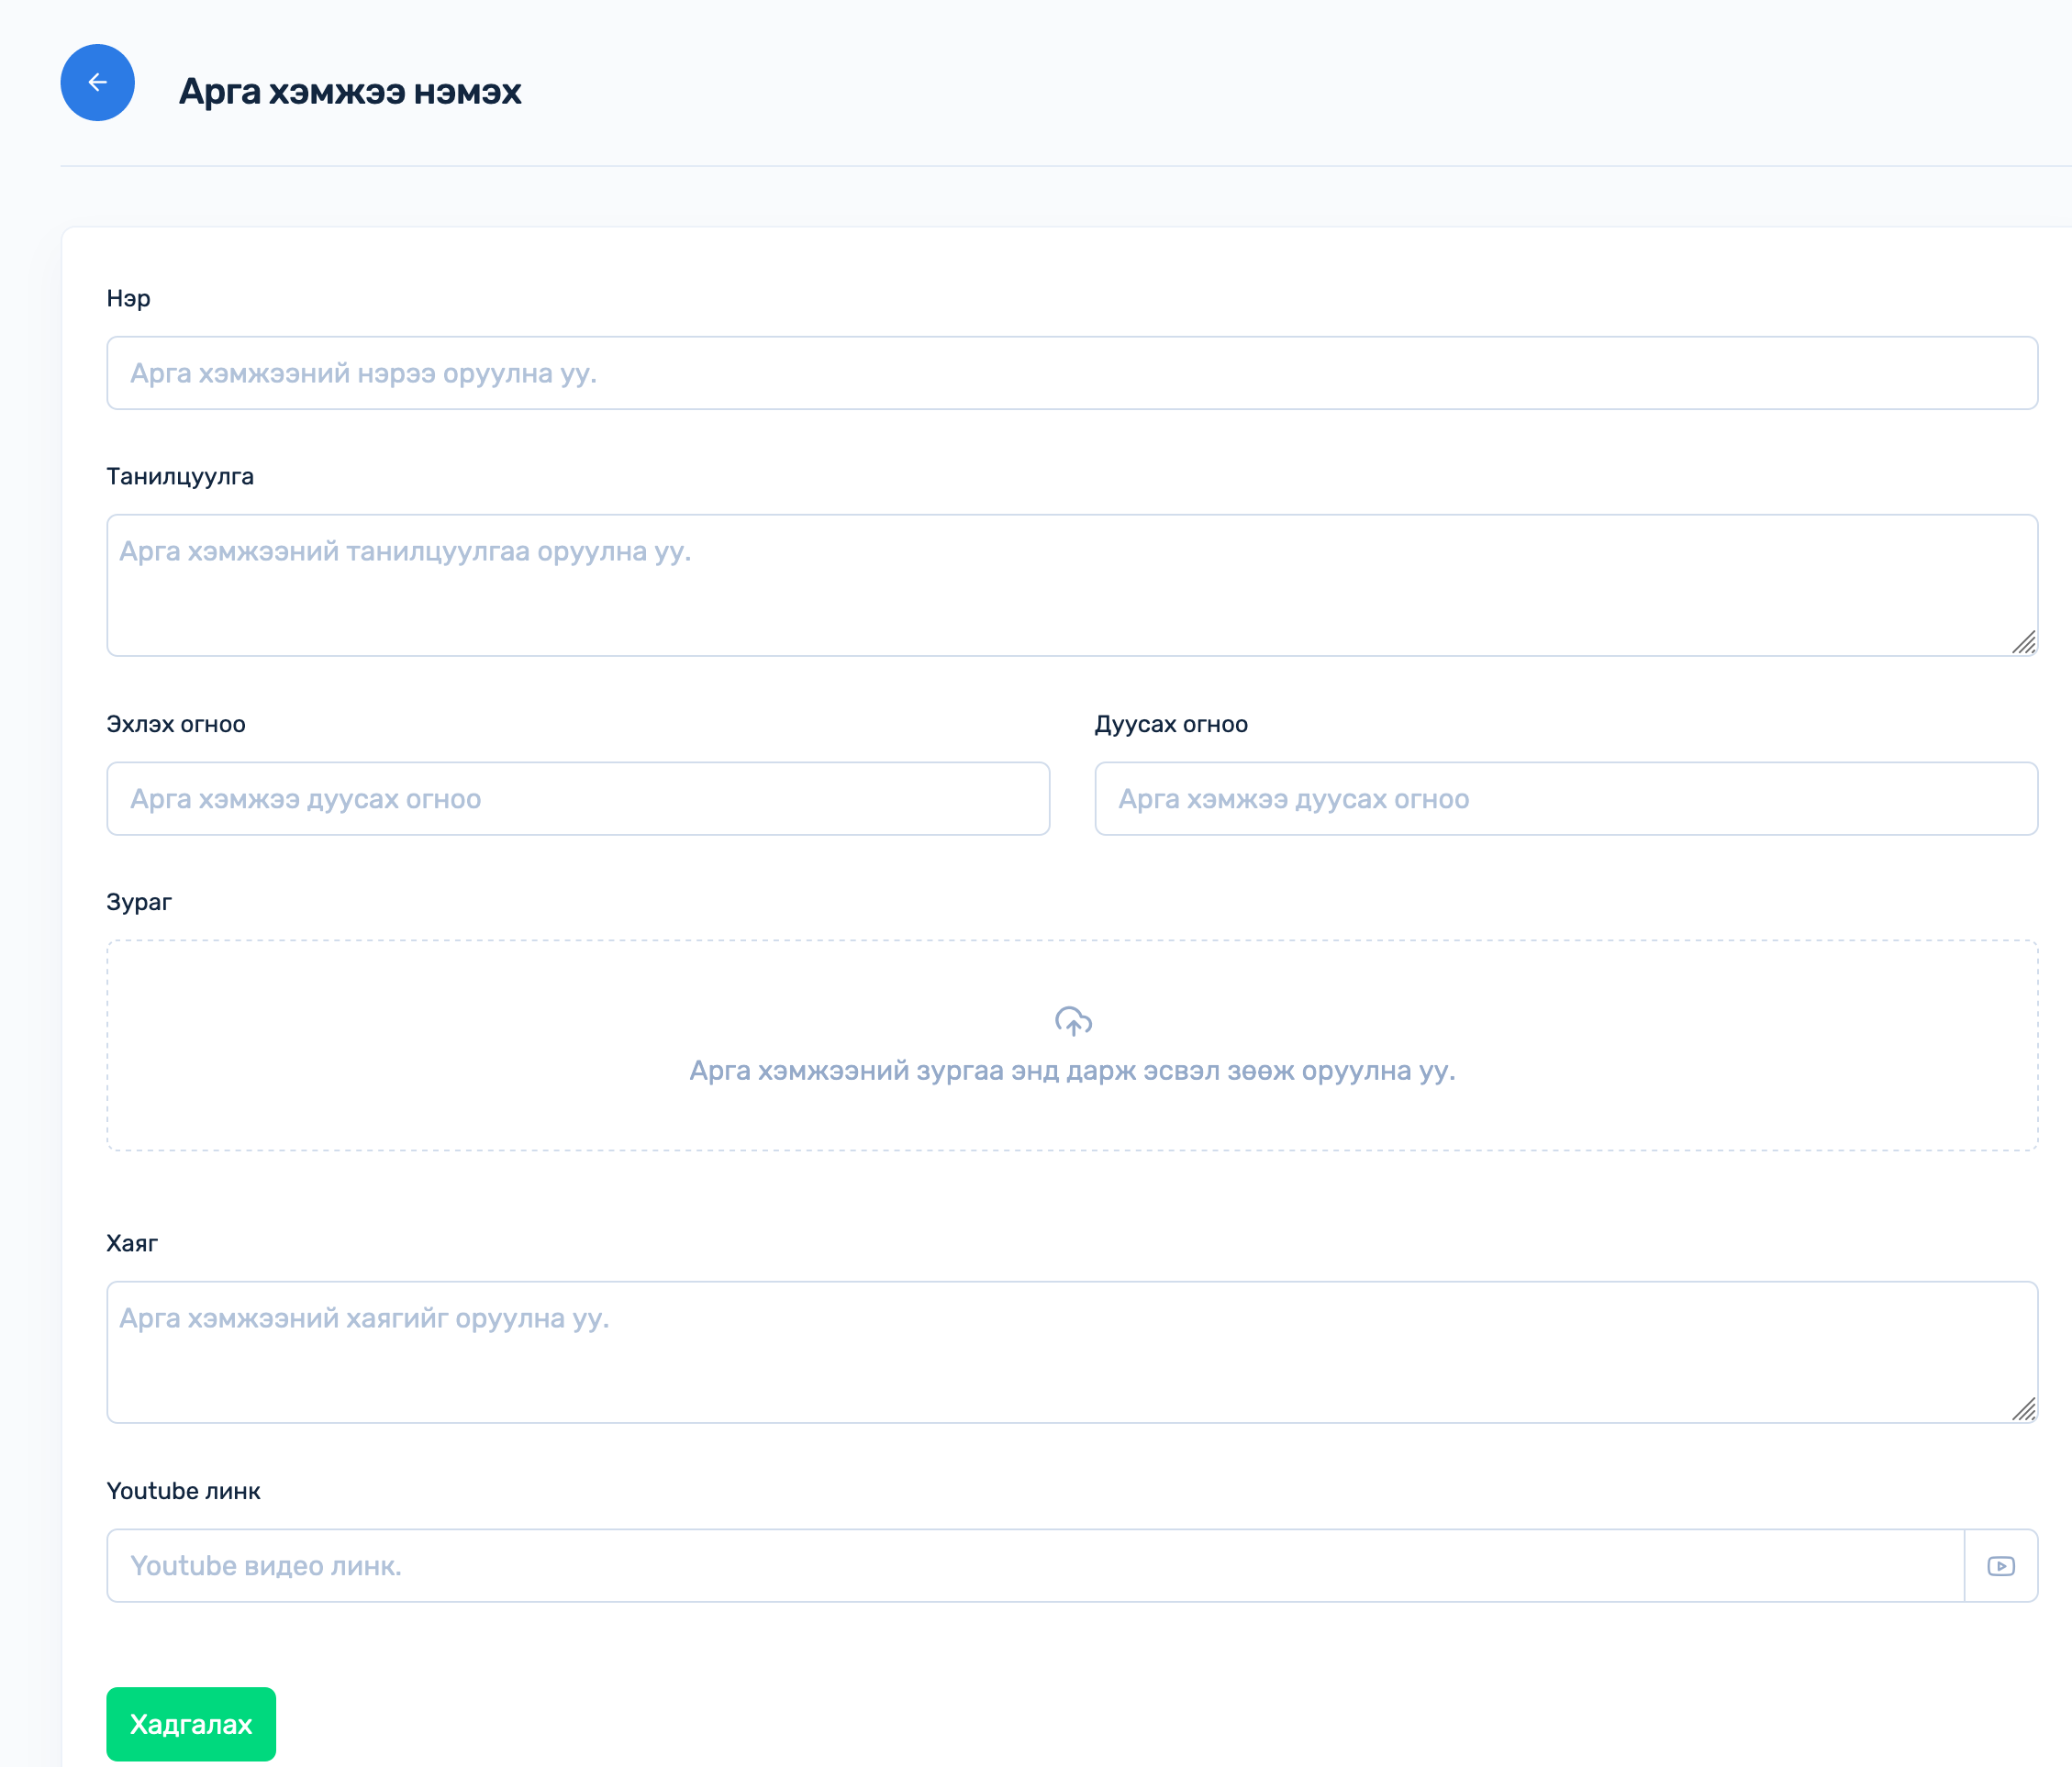
\includegraphics[scale=0.2]{src/images/event-form.png}
	\caption{Баннерийн форм хэсэг}
\end{figure}

\clearpage\section{Үйлчилгээний төлбөрийн саналын хуудас}
Zochil платформ шинээр үйлчилгээний төлбөрийн багц гаргаж байгаа бөгөөд Админ веб системд багц худалдаж аваагүй хэрэглэгчдэд саналын шинээр хуудас үүсгэх шаардлагатай болсон.
\lstinputlisting[language=Javascript, basicstyle=\linespread{0.8}\ttfamily, caption={Үйлчилгээний төлбөрийн саналын компонент},frame=single]{src/code/pricing/PricingPlan.js}

\subsection{Үр дүн}
\begin{figure}[h]
	\centering
	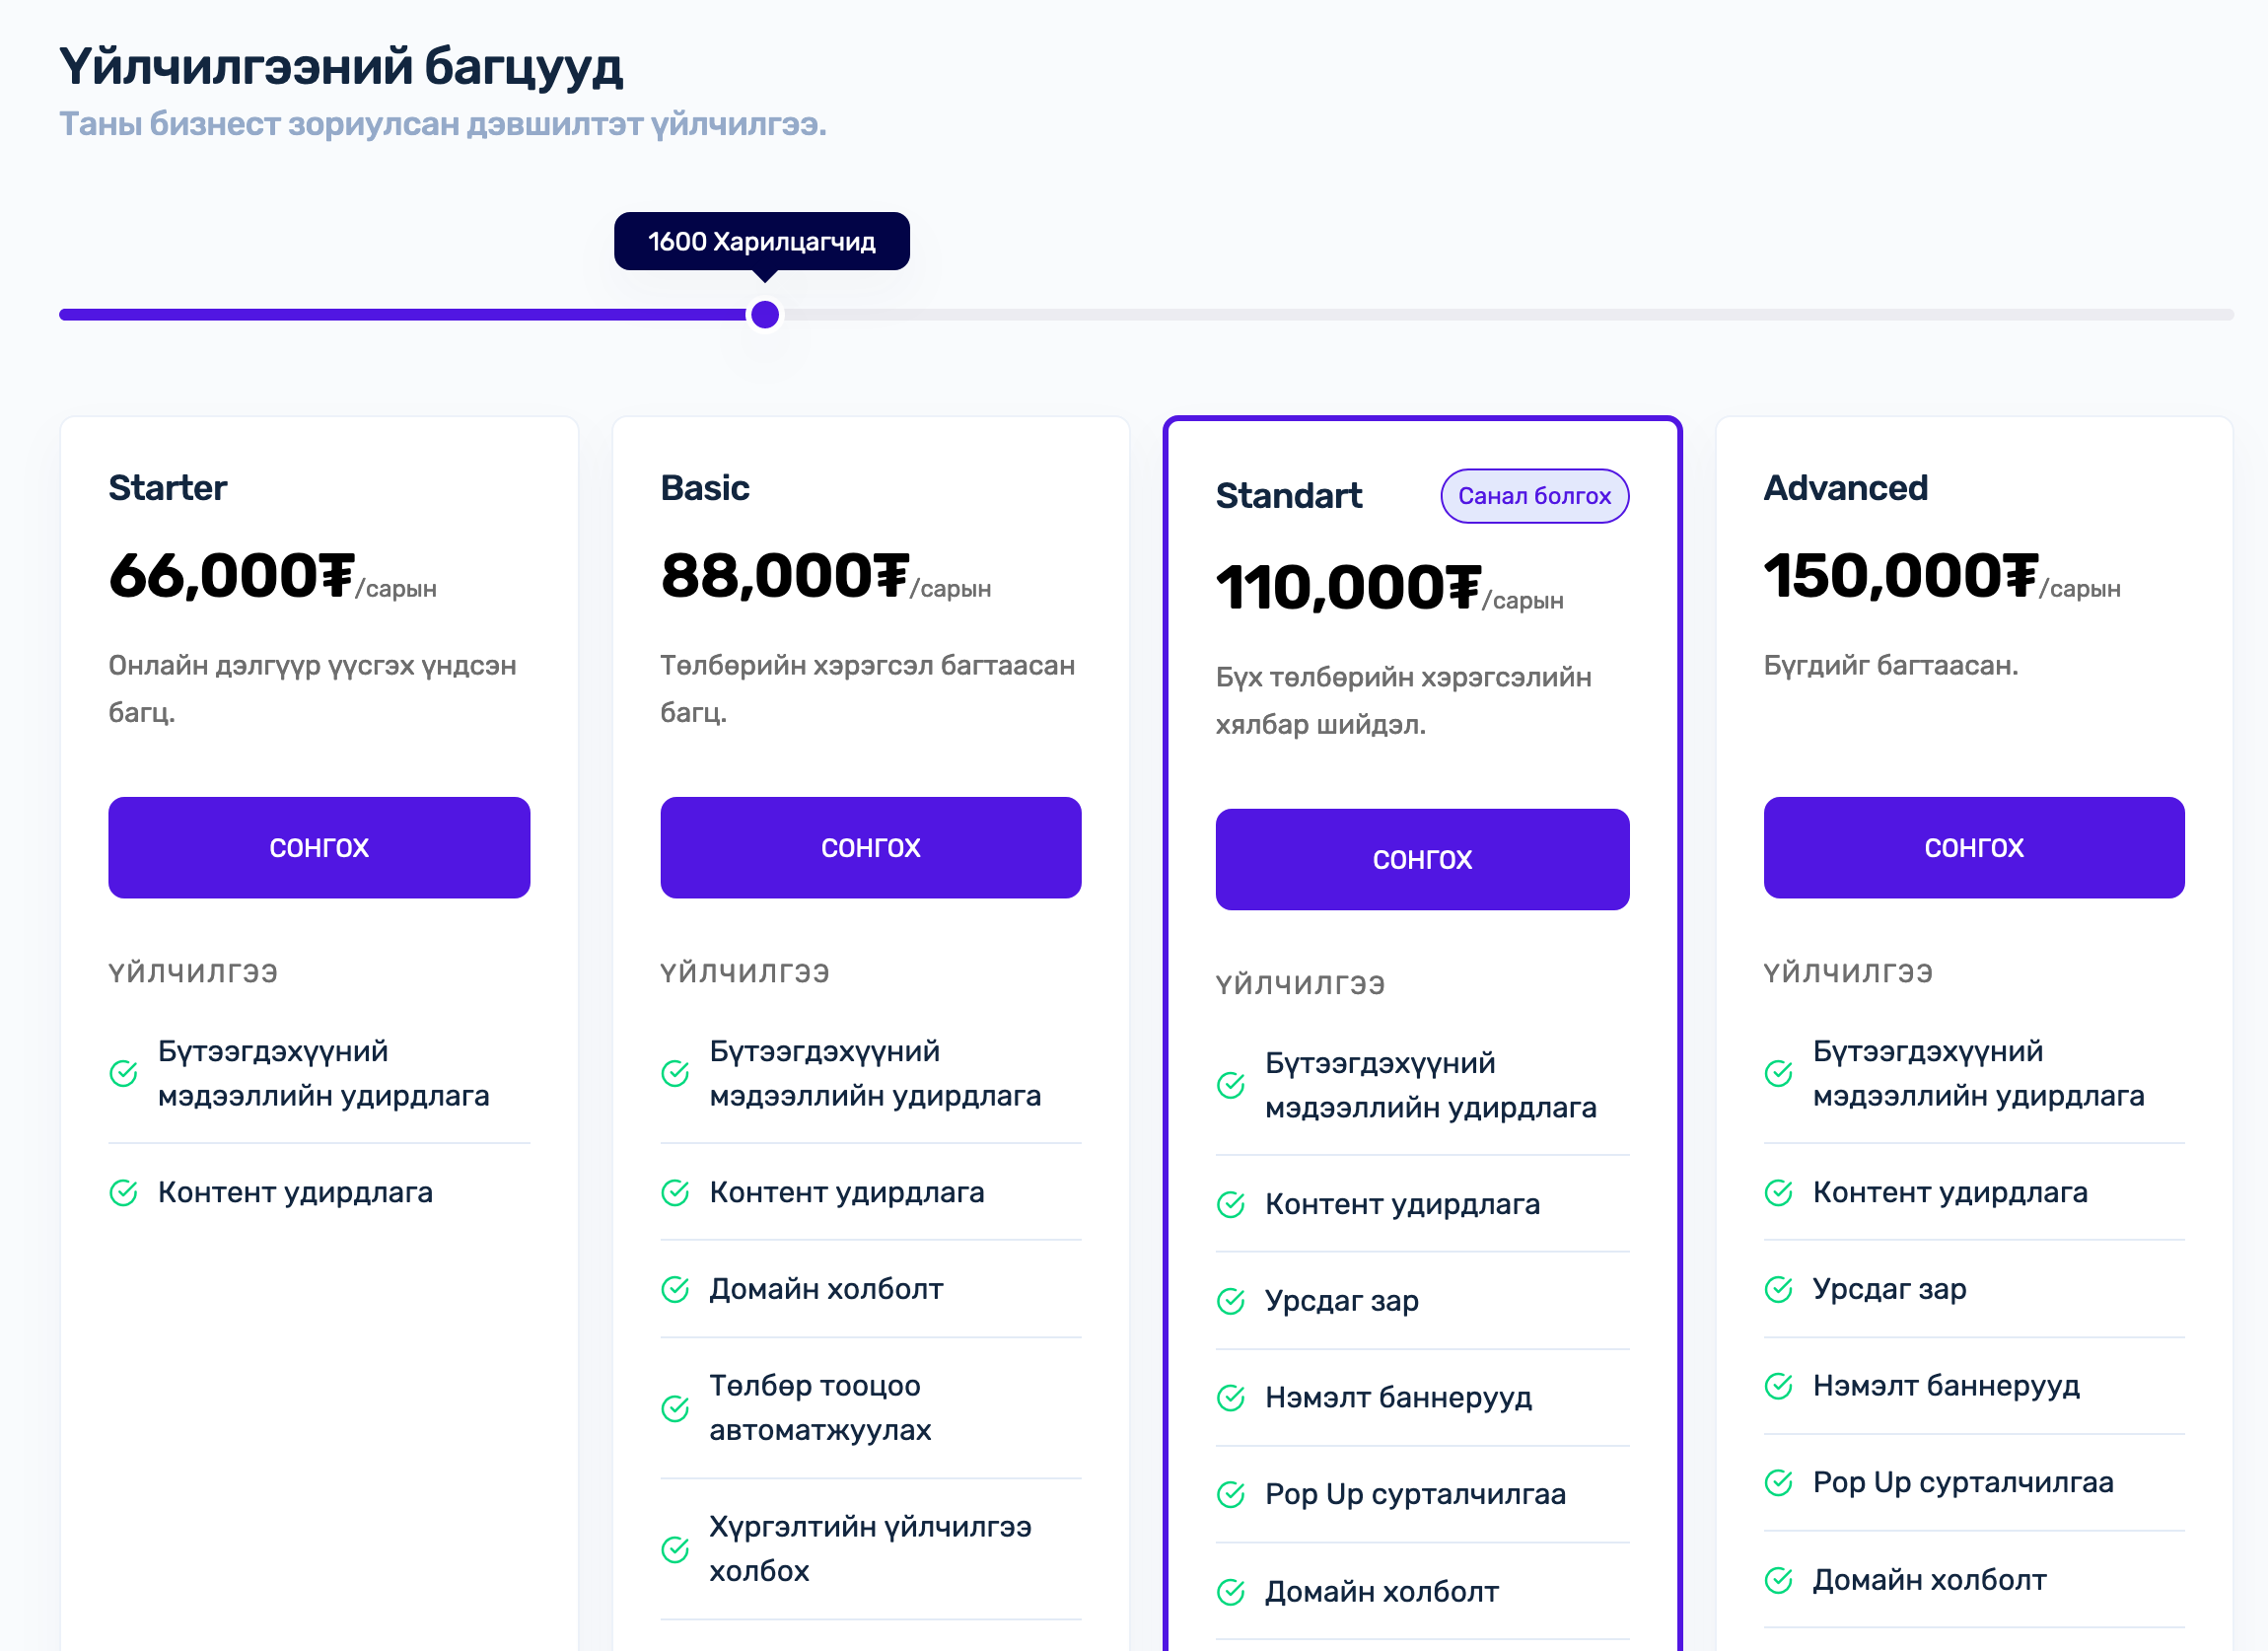
\includegraphics[scale=0.2]{src/images/pricing.png}
	\caption{Үйлчилгээний төлбөрийн саналын компонент}
\end{figure}

\section{Мод бүтэцтэй бүтээгдэхүүний категори}
\subsection{Өгөгдлийн сангаас категоруудыг авах custom hook}
\lstinputlisting[language=Javascript, basicstyle=\linespread{0.8}\ttfamily, caption={Категоруудыг авах  custom hook},frame=single]{src/code/category/UseMasterCategory.js}

\subsection{Фронтэнд хөгжүүлэлт}
\subsubsection{Категоруудыг нэмэх компонент}
\lstinputlisting[language=Javascript, basicstyle=\linespread{0.8}\ttfamily, caption={Категоруудыг нэмэх компонент},frame=single]{src/code/category/MasterCategory.js}
\subsubsection{Категоруудын жагсаалтын item компонент}
Категорууд нь мод бүтэцтэй учир нэг категори дотор хэдэн ч категори байж болно.
\lstinputlisting[language=Javascript, basicstyle=\linespread{0.8}\ttfamily, caption={Категоруудыг нэмэх компонент},frame=single]{src/code/category/MasterCategoryItem.js}

\subsection{Үр дүн}
\begin{figure}[h]
	\centering
	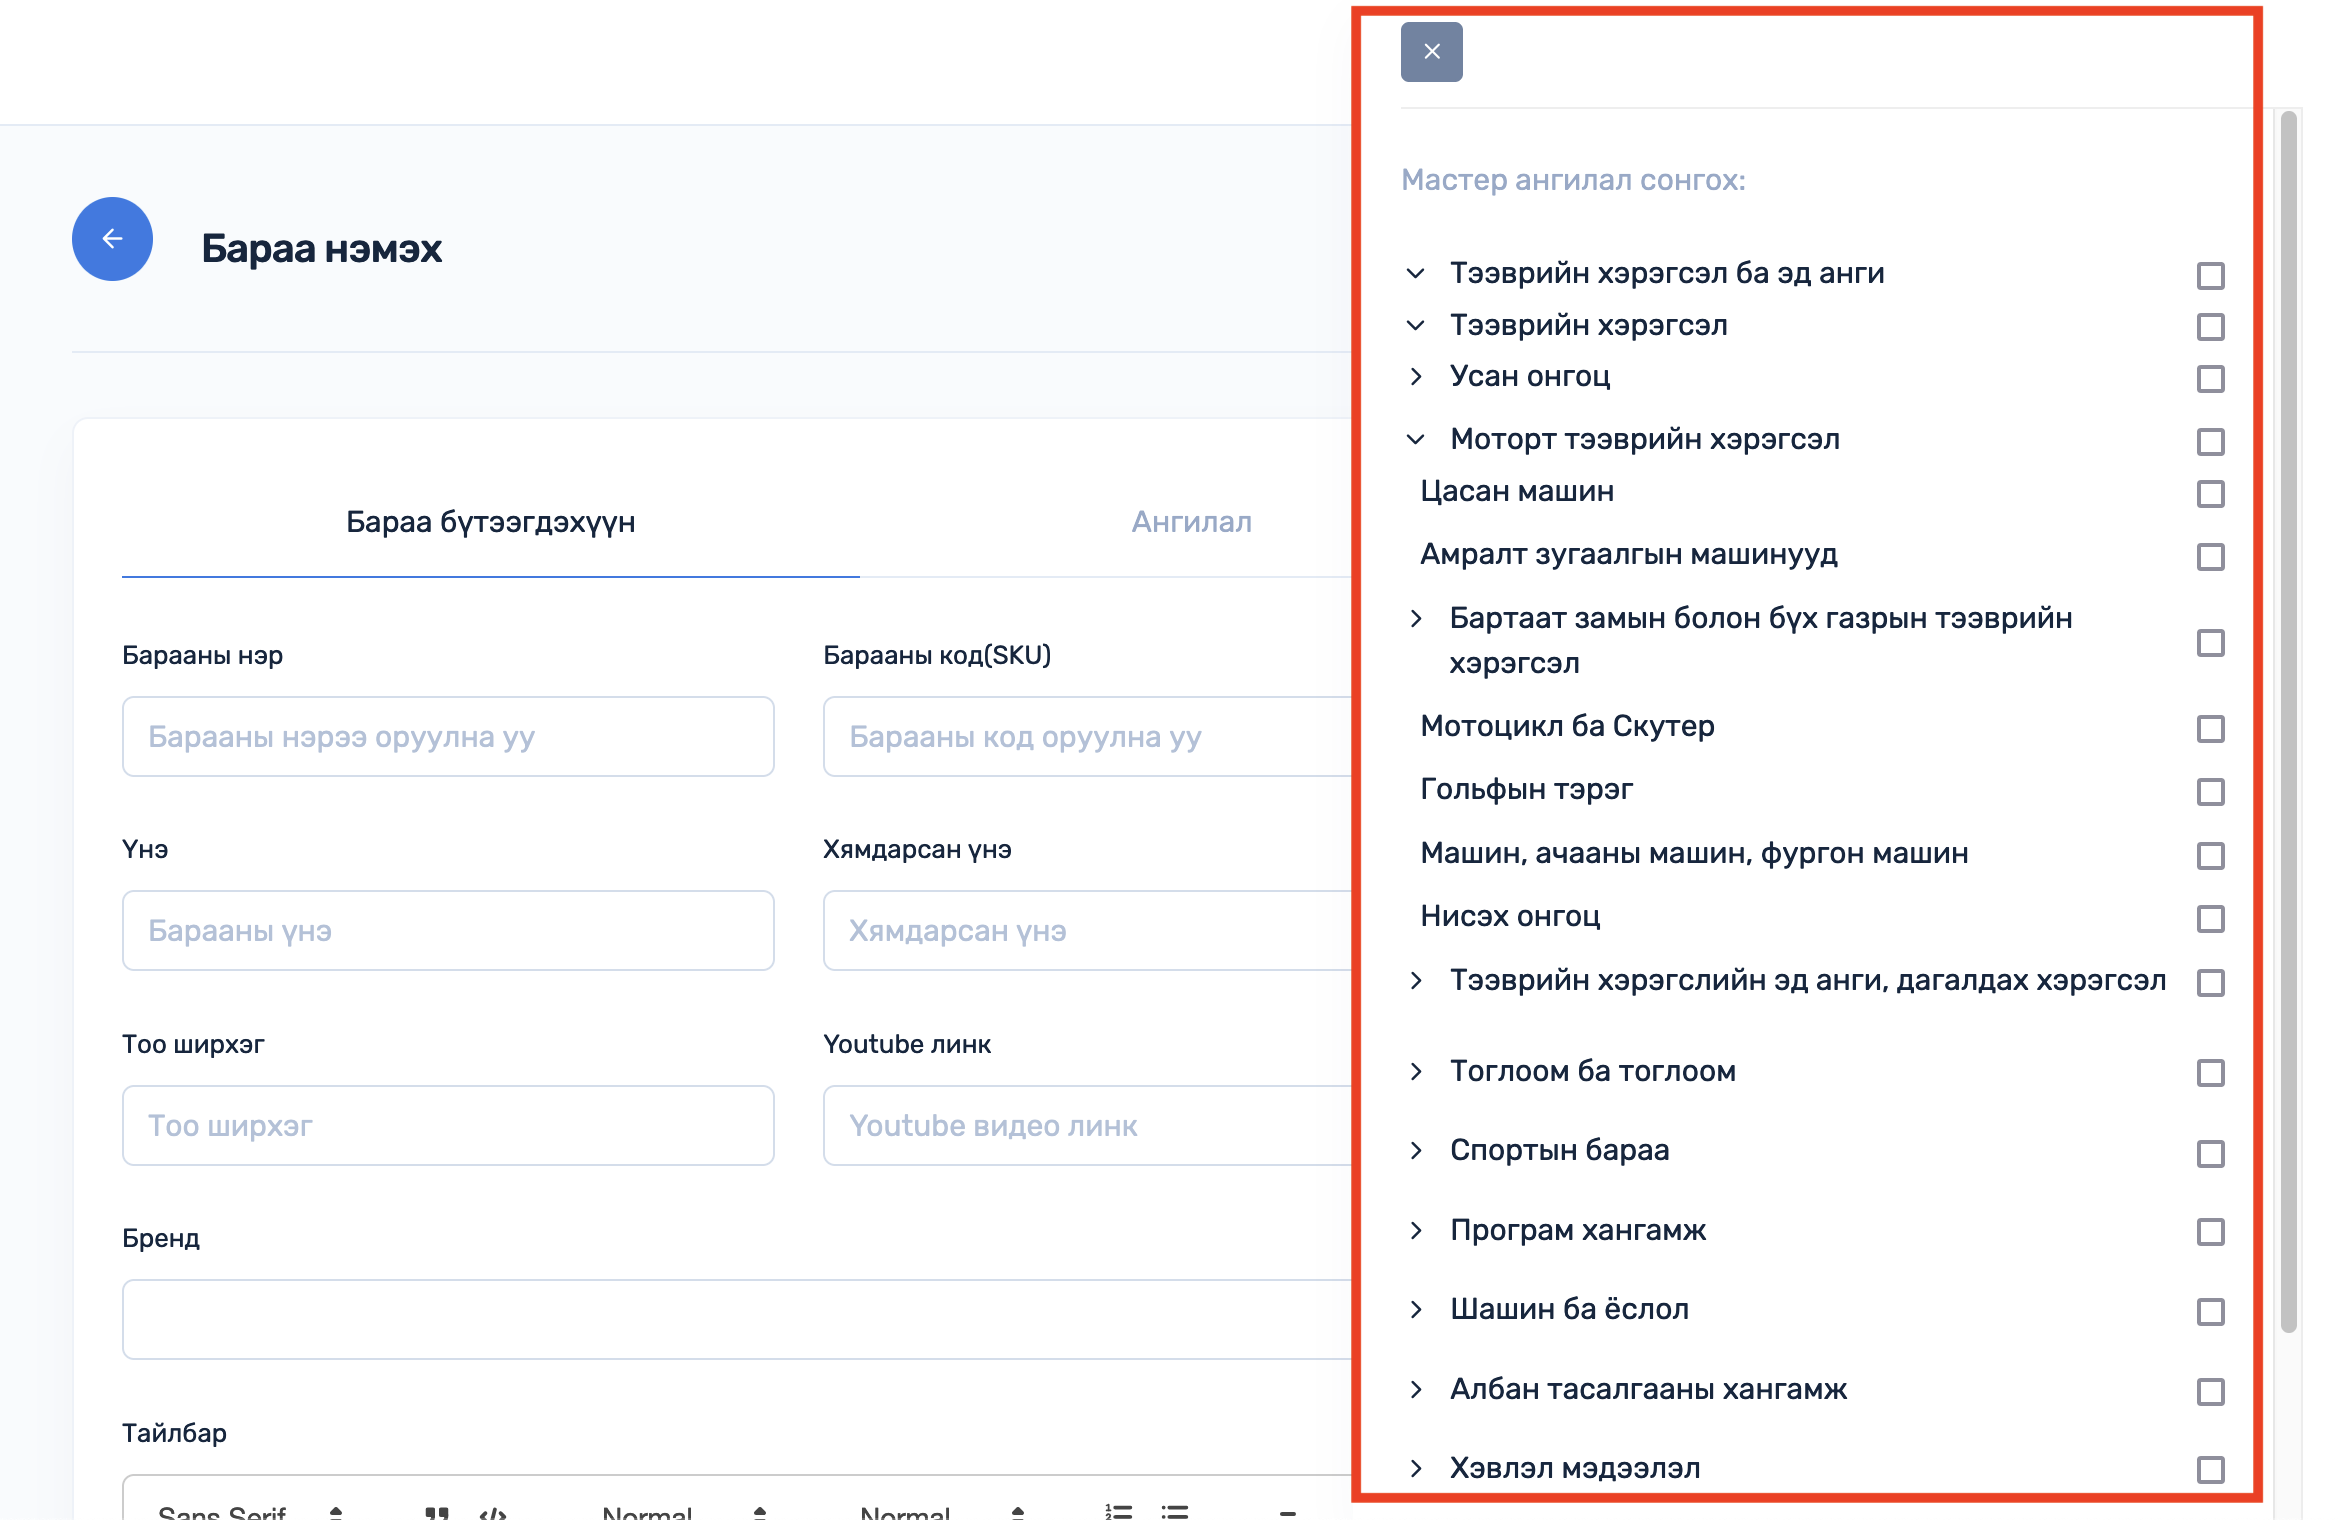
\includegraphics[scale=0.2]{src/images/category-add.png}
	\caption{Категоруудыг нэмэх компонент}
\end{figure}
